% Created 2021-01-24 Sun 22:50
% Intended LaTeX compiler: pdflatex
\documentclass[11pt]{article}
\usepackage[utf8]{inputenc}
\usepackage[T1]{fontenc}
\usepackage{graphicx}
\usepackage{grffile}
\usepackage{longtable}
\usepackage{wrapfig}
\usepackage{rotating}
\usepackage[normalem]{ulem}
\usepackage{amsmath}
\usepackage{textcomp}
\usepackage{amssymb}
\usepackage{capt-of}
\usepackage{hyperref}
\usepackage{minted}
\hypersetup{colorlinks=true, linkcolor=black, filecolor=red, urlcolor=blue}
\usepackage[turkish]{babel}
\author{Eren Hatırnaz}
\date{6 Ekim 2019}
\title{Yazılım Gündemi - 12\\\medskip
\large 30 Eylül - 6 Ekim 2019}
\hypersetup{
 pdfauthor={Eren Hatırnaz},
 pdftitle={Yazılım Gündemi - 12},
 pdfkeywords={},
 pdfsubject={},
 pdfcreator={Emacs 27.1 (Org mode 9.3)},
 pdflang={Turkish}}
\begin{document}

\maketitle
\tableofcontents \clearpage\shorthandoff{=}

\begin{center}
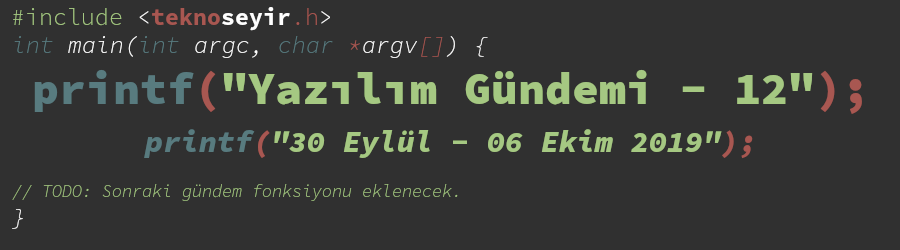
\includegraphics[width=.9\linewidth]{gorseller/yazilim-gundemi-banner.png}
\end{center}

\begin{center}
\href{../11/yazilim-gundemi-11.pdf}{< Önceki Gündem} | \textbf{30 Eylül - 06 Ekim 2019} | \href{../13/yazilim-gundemi-13.pdf}{Sonraki Gündem >}

\href{https://teknoseyir.com/blog/yazilim-gundemi-12-30-eylul-6-ekim-2019}{TeknoSeyir'de Oku}
\end{center}

\section{Yaklaşık 10 milyon proje \href{https://boyter.org/posts/an-informal-survey-of-10-million-github-bitbucket-gitlab-projects/}{analiz edildi}}
\label{sec:org5804e20}
\href{https://github.com/boyter/scc/}{scc} isimli kod satırı sayma ve karmaşıklık hesaplama aracının geliştiricisi Ben
E.C. Boyter, sunucu yardımıyla yaklaşık 40TB büyüklüğündeki toplamda 10 milyon
projeyi analiz etmiş ve detaylı bir blog yazısı hazırlamış. Go programlama
dilini kullanarak \$100 maliyetle (sanırım sunucu maliyeti) tüm bu işlemleri
yapabilmiş. Projeleri indirmesi toplam 5 hafta sürmüş. Bazı sonuçlar ise bu
şekilde:

\begin{itemize}
\item 9.985.051 toplam depo (repository),
\item 9.100.083 en az bir dosya bulunan depo,
\item 884.068 boş depo,
\item 3.500.000.000 tüm depoların toplam dosya sayısı,
\item 40.736.530.379.778 Byte (40TB) toplam işlenen veri,
\item 1.086.723.618.560 toplam satırı,
\item 816.822.273.469 toplam kod satırı,
\item 124.382.152.510 toplam boş satır,
\item 145.519.192.581 toplam yorum satırı.
\end{itemize}

Daha fazla istatistik ve ilginç veriler için mutlaka konu başlığına eklediğim
bağlantıya tıklayın.
\section{.NET Core 3.1 sürümünde \href{https://www.infoq.com/news/2019/10/CPP-CLI-NetCore/}{C++ desteği gelecek}}
\label{sec:org2ce2d7d}
Aslında bu haber geçen haftanın konusu fakat .NET 3.0 duyulunca sanırım bu
haber arkaplanda kalmış olacak ki konu başlığına eklediğim site de bunu 3 ekim
tarihinde haber yapmış. Biliyorsunuz Microsoft çok uzun zamandır .NET Framework
sistemi üzerinde duruyordu fakat yeni CEO Satya Nadella ile açık kaynak
dünyasına girmeye yönelik birçok adım attı Microsoft ve Visual Studio Code ve
.NET Core gibi projelere imza attı. .NET Core, .NET Framework olarak birliğimiz
uygulama çatısının açık kaynak ve platformlar arası (cross-platform) hale
gelmiş sürümü diyebiliriz. Bu sayede .NET ekosistemi hem açık kaynak camiasında
bir topluluk oluşturdu hem de GNU/Linux dağıtımları ve Mac sistemlerde .NET
uygulaması geliştirme imkanı doğdu. Bu sefer de Microsoft \href{https://devblogs.microsoft.com/cppblog/the-future-of-cpp-cli-and-dotnet-core-3/}{bloglarında
yayınladıkları bir yazı} ile .NET Core 3.1 sürümünde C++ ile Windows uygulaması
geliştirme desteğinin geleceğini duyurdu. Windows uygulaması olduğu için
haliyle GNU/Linux ve Mac sistemlerde bu özellikten faydalanılamayacak olsa da
ileride tüm uygulamalar için de C++ desteği gelebilir. Bakalım süreç nasıl
ilerleyecek.
\section{İngiltere RESTful API standardı için \href{https://technology.blog.gov.uk/2019/10/02/improve-csvs-and-api-descriptions-with-these-open-standards-board-recommendations/}{OpenAPI 3 öneriyor}}
\label{sec:org2b4808a}
Açık kaynak artık öyle bir noktaya geldi ki, artık devletler bile bu ekosisteme
katkı vermeye başladı. İngiltere'de birkaç yıldır bu akıma ayak uyduran
ülkelerden birisi, hatta yanlış hatırlamıyorsam bu akımı başlatan ülke bile
olabilir. İngiltere'nin ilgili kurumunun içerisindeki Açık Standartlar
Kurulu'da (Open Standards Boards), devlet içerisindeki geliştirmelerde
kullanılacak standartları belirlemeye çalışıyor. Kurulun GitHub üzerindeki
deposuna \href{https://github.com/alphagov/open-standards/issues/31}{gönderilen} "API tanımlamaları için OpenAPI kullanalım" konulu öneri de
kurul tarafından tartışılmış ve kabul edilmiş. OpenAPI ise, RESTful API
geliştirmelerinde sistemin yapısını kurarken baz alınabilecek çeşitli
tanımlamaları ve kuralları olan bir standart. Artık İngiltere'de devlet
tarafından önerilen bir standart oldu.

Böyle şeyler gördükçe insan imreniyor tabii.
\section{WhiteSource firması, \href{https://www.whitesourcesoftware.com/developers-security-report/}{uygulama güvenliği anketi sonuçları}nı yayınladı}
\label{sec:orgbea8762}
WhiteSource isimli güvenlik firmasının yaklaşık 600 geliştirici ile yaptığı
uygulama güvenliği anketinin sonuçlardan bir kısım şu şekilde:
\subsection{Şirketinizde uygulama güvenliğinden kim(ler) sorumlu?}
\label{sec:orgfe3e1f0}
\begin{center}
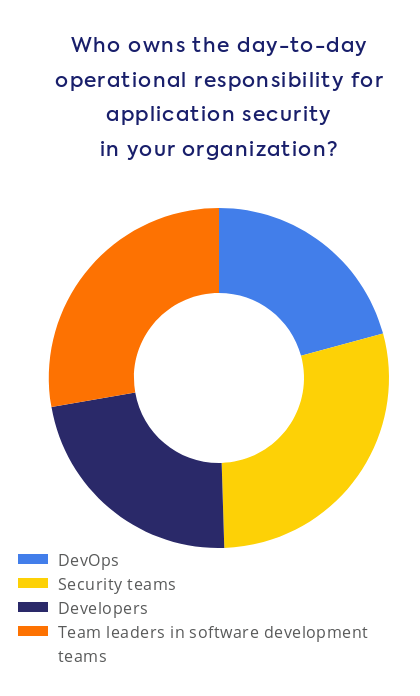
\includegraphics[height=6cm]{gorseller/anket-1.png}
\end{center}

Pastadaki en büyük pay \%29 ile güvenlik takımları almış. Açıkcası bir
geliştirici olarak güvenlik konuları için artık özel takımlar oluşturulması
beni mutlu etti. Elbette geliştiriciler olarak yazdığımız kodlardaki güvenlik
açıklarından sorumluyuz fakat bunların tespiti için ayrı bir takım gerekli
bence. Öbür türlü üzerimizde çok fazla yük bindiriliyormuş gibi hissediyorum.
\subsection{Şirket büyüklerine göre güvenlikten kim(ler) sorumlu}
\label{sec:org8215bd9}
\begin{center}
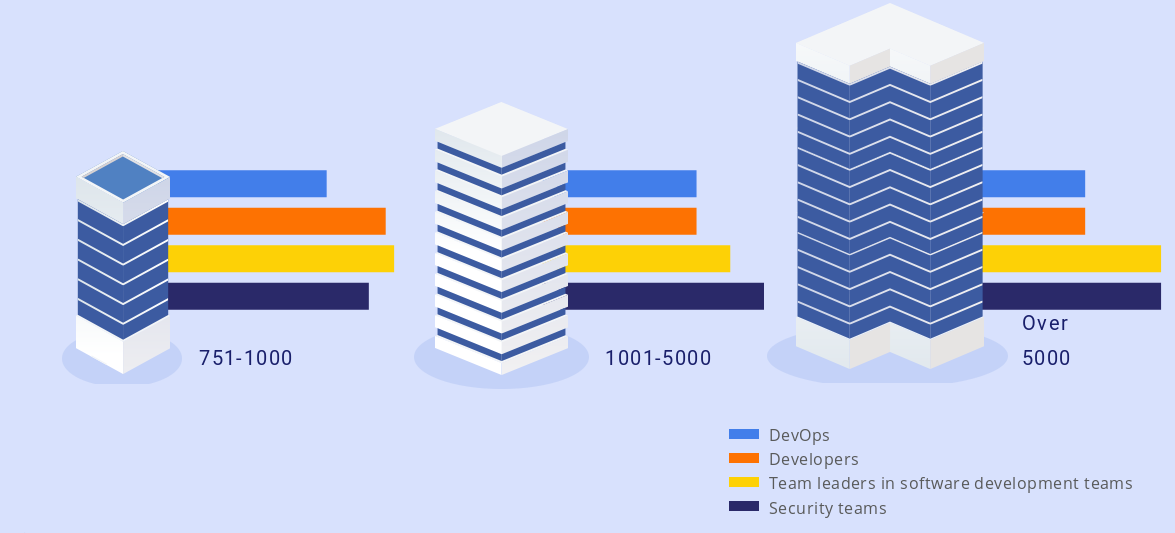
\includegraphics[width=.9\linewidth]{gorseller/anket-2.png}
\end{center}

Anketin diğer sonuçları için mutlaka konu başlığına eklediğim bağlantıya
tıklayın. Uygulama ve dolayısıyla verilerin güvenliği günümüzde önemi hızla
artan konulardan birisi.
\section{Etkinlik Duyurusu: \href{https://kommunity.com/atolye15/events/lifecycle-of-a-product-with-scrum}{Lifecycle of a Product with Scrum}}
\label{sec:orga42626d}
\begin{center}
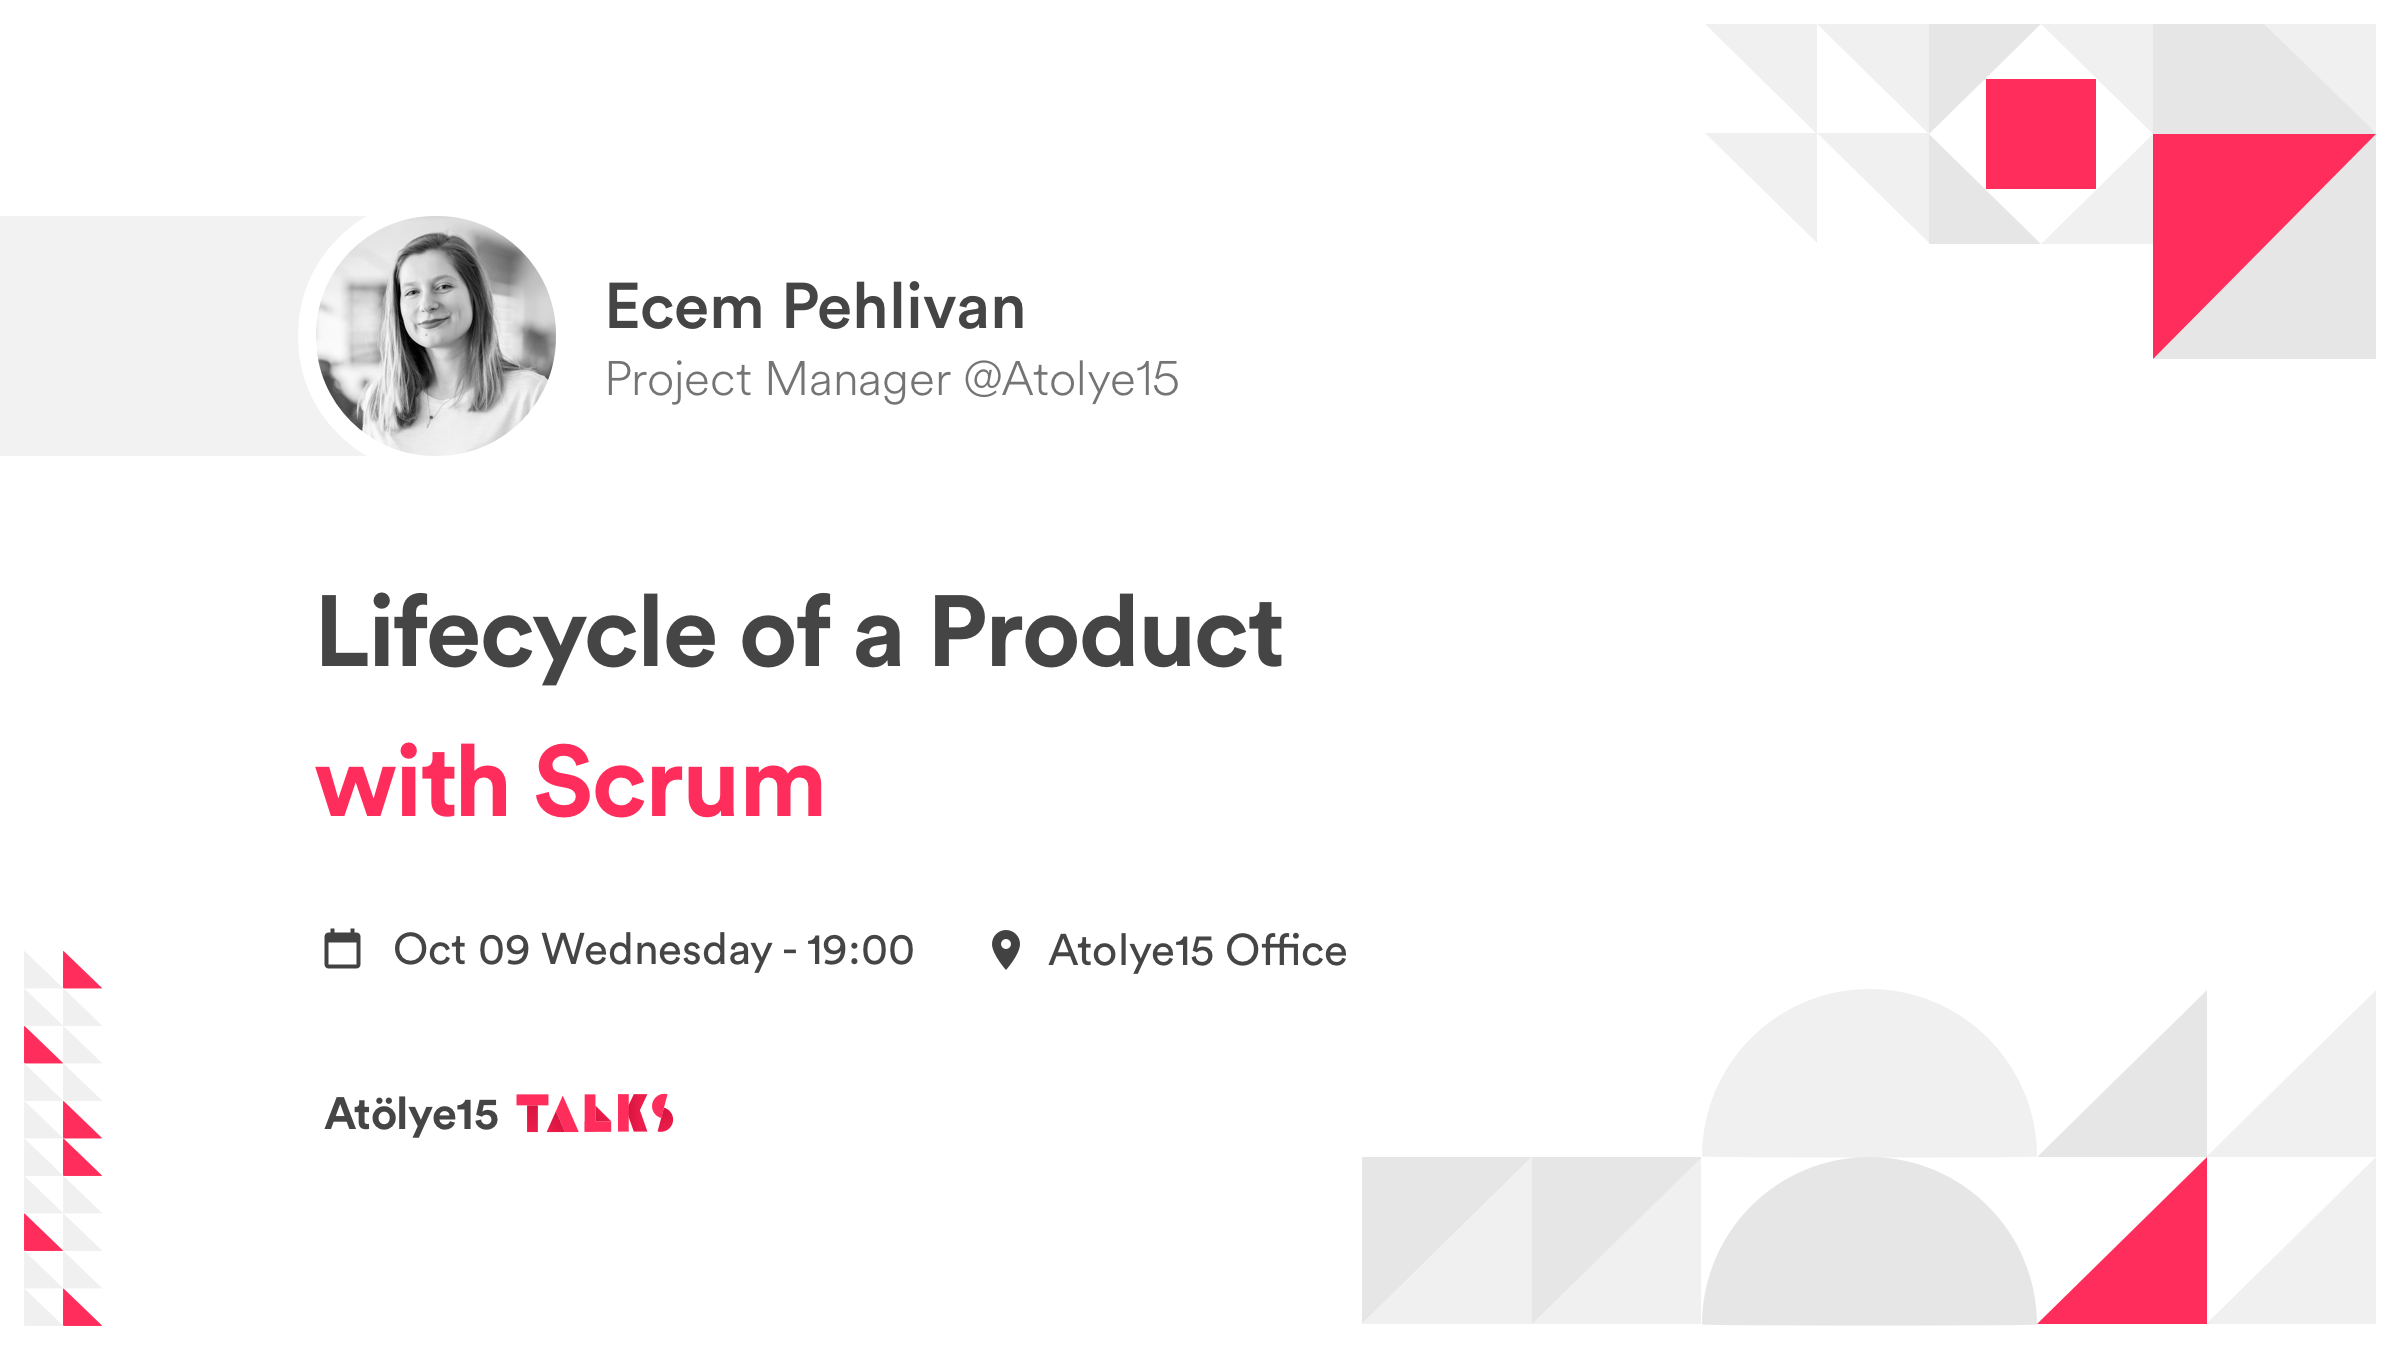
\includegraphics[width=.9\linewidth]{gorseller/ecem-meetup.png}
\end{center}
\section{Diğer Haberler}
\label{sec:org472eeaf}
\begin{itemize}
\item TypeScript \href{https://devblogs.microsoft.com/typescript/announcing-typescript-3-7-beta/}{3.7 Beta sürecine girdi}.
\item Xilinx firması, gömülü sistem programcıları için yeni bir \href{https://www.xilinx.com/news/press/2019/xilinx-announces-vitis--a-unified-software-platform-unlocking-a-new-design-experience-for-all-developers.html}{uygulama platformu
duyurdu}: \href{https://www.xilinx.com/products/design-tools/vitis.html}{Vitis}. \href{https://www.eejournal.com/article/xilinx-vitis-and-vitis-ai-software-development-platforms/}{Alternatif}
\item Google Cloud Platform takımı yeni bir Kubernetes \href{https://www.ververica.com/blog/google-cloud-platforms-flink-operator-for-kubernetes}{aracı duyurdu}:
\href{https://github.com/GoogleCloudPlatform/flink-on-k8s-operator}{flink-on-k8n-operator}.
\item Google, Linux çekirdeğine katkı olarak üzerinde çalıştığı sanitizer
projesini \href{https://www.phoronix.com/scan.php?page=news\_item\&px=Google-KCSAN-Sanitizer}{açık kaynak yaptı}: \href{https://github.com/google/ktsan}{Kernel Concurrency Sanitizer (KCSAN)}
\item Linux'deki yeni bellek kontrolcüsü \href{https://thenewstack.io/a-new-linux-memory-controller-promises-to-save-lots-of-ram/}{RAM tasarrufu sağlıyormuş}.
\item Go ile yazılmış web sunucusu \href{https://github.com/caddyserver/caddy}{caddy} tüm projelerini \href{https://github.com/caddyserver/caddy/issues/2786}{açık kaynak lisanslara
geçirmeyi planlıyor}.
\item Derin öğrenme yöntemleri sayesinde hayvanların davranışlarını inceleyen yeni
\href{https://www.nature.com/articles/d41586-019-02942-5}{açık kaynak araçlar geliştiriliyormuş}.
\item Makine öğrenmesi ve veri bilimiyle uğraşanlar için \href{https://towardsdatascience.com/coding-ml-tools-like-you-code-ml-models-ddba3357eace}{yeni bir uygulama çatısı
(freamework) duyuruldu}: \href{https://streamlit.io/}{Streamlit}. \href{https://github.com/streamlit/streamlit}{GitHub Deposu}.
\item Makine öğrenmesi uygulamalarında sıkça kullanılan Python kütüphanesi
Tensorflow \href{https://github.com/tensorflow/tensorflow/releases/tag/v2.0.0}{2.0.0 sürümü duyuruldu}.
\item 3.parti GitHub mobil uygulaması GitTouch \href{https://github.com/pd4d10/git-touch/releases/tag/v1.1.0}{1.1.0 sürümünü çıkardı}. \href{https://itunes.apple.com/us/app/gittouch/id1452042346}{Apple
Market}, \href{https://play.google.com/store/apps/details?id=io.github.pd4d10.gittouch}{Google Play}.
\item PostgreSQL \href{https://www.postgresql.org/about/news/1976/}{12 sürümü yayınlandı}.
\item SQLite veritabanının \href{https://www.sqlite.org/changes.html}{3.30.0 sürümünü duyuruldu}.
\item Zig programlama dilinin \href{https://ziglang.org/download/0.5.0/release-notes.html}{0.5.0 sürümü duyuruldu}.
\item Lua programlama dilinin \href{http://lua-users.org/lists/lua-l/2019-10/msg00003.html}{5.4.0 sürümü duyuruldu}.
\item Inko programlama dilinin \href{https://inko-lang.org/news/inko-progress-report-september-2019/}{Eylül ayı durum raporu yayınlandı}.
\item NextJS, \href{https://nextjs.org/blog/next-9-0-7}{9.0.7 sürümü çıktı}.
\item API Platform \href{https://dunglas.fr/2019/09/api-platform-2-5-revamped-admin-new-api-testing-tool-next-js-and-quasar-app-generators-patch-and-json-schema-support-improved-openapi-and-graphql-support}{2.5 sürümü çıktı}.
\item Rust kütüphanesi \texttt{static-assertions} ilk \href{https://nikolaivazquez.com/posts/programming/rust-static-assertions-1\_0/}{stabil sürümü 1.0.0'ı duyurdu}.
\end{itemize}
\section{Lisans}
\label{sec:orgc14ca4a}
\begin{center}
\begin{center}

\includegraphics[height=1.5cm]{../../../img/CC_BY-NC-SA_4.0.png}
\end{center}

\href{yazilim-gundemi-12.pdf}{Yazılım Gündemi - 12} yazısı \href{https://erenhatirnaz.github.io}{Eren Hatırnaz} tarafından \href{http://creativecommons.org/licenses/by-nc-sa/4.0/}{Creative Commons
Atıf-GayriTicari-AynıLisanslaPaylaş 4.0 Uluslararası Lisansı} (CC BY-NC-SA 4.0)
ile lisanslanmıştır.
\end{center}
\end{document}
